\newcommand{\gptpart}{10}
\newcommand{\gpttitle}{Practical Exploration of Advanced Concepts}
\newcommand{\gptsubtitle}{Translating Graviton Dynamics into Testable and Applied Realities}
\newcommand{\gptdate}{November 2026}
% Shared preamble for the second edition of Graviton Pressure Theory.
% A part's own file sets \gptpart, \gpttitle, \gptsubtitle and \gptdate, then % Shared preamble for the second edition of Graviton Pressure Theory.
% A part's own file sets \gptpart, \gpttitle, \gptsubtitle and \gptdate, then % Shared preamble for the second edition of Graviton Pressure Theory.
% A part's own file sets \gptpart, \gpttitle, \gptsubtitle and \gptdate, then \input{../common/preamble}.
\documentclass[11pt,a4paper]{article}
\usepackage[T1]{fontenc}
\usepackage[utf8]{inputenc}
\usepackage{mathpazo}
\usepackage[scaled=0.92]{helvet}
\usepackage{amsmath,amssymb}
\usepackage[margin=2.5cm]{geometry}
\usepackage{microtype}
\usepackage{graphicx}
\usepackage{booktabs,array,tabularx}
\usepackage[font=small,labelfont=bf]{caption}
\usepackage{enumitem}
\usepackage[authoryear,round]{natbib}
\usepackage{titlesec}
\usepackage[titles]{tocloft}
\renewcommand{\cftsecfont}{\bfseries}\renewcommand{\cftsecpagefont}{\bfseries}
\renewcommand{\cftsecleader}{\hfill}\setlength{\cftsecnumwidth}{3.2em}
\usepackage{gpt-status}
\usepackage[hidelinks]{hyperref}
\setlength{\parskip}{4pt}
\setlength{\emergencystretch}{3em}
\setlength{\parindent}{0pt}
\setlist{itemsep=2pt,topsep=3pt}
\titleformat{\section}{\Large\bfseries}{\thesection}{1em}{}
\titleformat{\subsection}{\large\bfseries}{\thesubsection}{1em}{}
\renewcommand{\thesection}{\gptpart.\arabic{section}}
\renewcommand{\thetable}{\gptpart.\arabic{table}}
\renewcommand{\thefigure}{\gptpart.\arabic{figure}}
\renewcommand{\theequation}{\gptpart.\arabic{equation}}
\setcounter{tocdepth}{1}
\makeatletter\renewcommand{\@pnumwidth}{2.2em}\renewcommand{\@tocrmarg}{3em}
\makeatother
\bibliographystyle{plainnat}
\newcommand{\gptitle}{%
  \begin{titlepage}\centering
  \vspace*{3cm}
  {\Huge\bfseries Graviton Pressure Theory\par}\vspace{0.8cm}
  {\Large The Unified Framework\par}\vspace{0.2cm}
  {\large Individual Submission\par}\vspace{0.6cm}
  {\normalsize This document is part of a multi-part scientific framework\par}\vspace{2cm}
  {\normalsize Part \gptpart\ of 30\par}\vspace{0.8cm}
  {\huge\bfseries \gpttitle\par}\vspace{0.6cm}
  {\Large \gptsubtitle\par}\vspace{1.5cm}
  {\small\begin{minipage}{0.75\textwidth}\centering This submission is part of the broader Graviton Pressure Theory (GPT) project, a redefinition of gravitational interaction rooted in causal field dynamics and physical force transmission. Each document is designed to stand on its own; its full context emerges as part of the larger framework. For the complete series, see https://peopleoftheworld.net/graviton-pressure-theory/.\end{minipage}\par}
  \vfill
  {\large Author: Shareef Ali Rashada\par}\vspace{0.2cm}
  {\normalsize shareef@peopleoftheworld.net\par}\vspace{0.5cm}
  {\normalsize Second edition, \gptdate\par}
  \end{titlepage}
  \setcounter{page}{1}\tableofcontents\clearpage}
.
\documentclass[11pt,a4paper]{article}
\usepackage[T1]{fontenc}
\usepackage[utf8]{inputenc}
\usepackage{mathpazo}
\usepackage[scaled=0.92]{helvet}
\usepackage{amsmath,amssymb}
\usepackage[margin=2.5cm]{geometry}
\usepackage{microtype}
\usepackage{graphicx}
\usepackage{booktabs,array,tabularx}
\usepackage[font=small,labelfont=bf]{caption}
\usepackage{enumitem}
\usepackage[authoryear,round]{natbib}
\usepackage{titlesec}
\usepackage[titles]{tocloft}
\renewcommand{\cftsecfont}{\bfseries}\renewcommand{\cftsecpagefont}{\bfseries}
\renewcommand{\cftsecleader}{\hfill}\setlength{\cftsecnumwidth}{3.2em}
\usepackage{gpt-status}
\usepackage[hidelinks]{hyperref}
\setlength{\parskip}{4pt}
\setlength{\emergencystretch}{3em}
\setlength{\parindent}{0pt}
\setlist{itemsep=2pt,topsep=3pt}
\titleformat{\section}{\Large\bfseries}{\thesection}{1em}{}
\titleformat{\subsection}{\large\bfseries}{\thesubsection}{1em}{}
\renewcommand{\thesection}{\gptpart.\arabic{section}}
\renewcommand{\thetable}{\gptpart.\arabic{table}}
\renewcommand{\thefigure}{\gptpart.\arabic{figure}}
\renewcommand{\theequation}{\gptpart.\arabic{equation}}
\setcounter{tocdepth}{1}
\makeatletter\renewcommand{\@pnumwidth}{2.2em}\renewcommand{\@tocrmarg}{3em}
\makeatother
\bibliographystyle{plainnat}
\newcommand{\gptitle}{%
  \begin{titlepage}\centering
  \vspace*{3cm}
  {\Huge\bfseries Graviton Pressure Theory\par}\vspace{0.8cm}
  {\Large The Unified Framework\par}\vspace{0.2cm}
  {\large Individual Submission\par}\vspace{0.6cm}
  {\normalsize This document is part of a multi-part scientific framework\par}\vspace{2cm}
  {\normalsize Part \gptpart\ of 30\par}\vspace{0.8cm}
  {\huge\bfseries \gpttitle\par}\vspace{0.6cm}
  {\Large \gptsubtitle\par}\vspace{1.5cm}
  {\small\begin{minipage}{0.75\textwidth}\centering This submission is part of the broader Graviton Pressure Theory (GPT) project, a redefinition of gravitational interaction rooted in causal field dynamics and physical force transmission. Each document is designed to stand on its own; its full context emerges as part of the larger framework. For the complete series, see https://peopleoftheworld.net/graviton-pressure-theory/.\end{minipage}\par}
  \vfill
  {\large Author: Shareef Ali Rashada\par}\vspace{0.2cm}
  {\normalsize shareef@peopleoftheworld.net\par}\vspace{0.5cm}
  {\normalsize Second edition, \gptdate\par}
  \end{titlepage}
  \setcounter{page}{1}\tableofcontents\clearpage}
.
\documentclass[11pt,a4paper]{article}
\usepackage[T1]{fontenc}
\usepackage[utf8]{inputenc}
\usepackage{mathpazo}
\usepackage[scaled=0.92]{helvet}
\usepackage{amsmath,amssymb}
\usepackage[margin=2.5cm]{geometry}
\usepackage{microtype}
\usepackage{graphicx}
\usepackage{booktabs,array,tabularx}
\usepackage[font=small,labelfont=bf]{caption}
\usepackage{enumitem}
\usepackage[authoryear,round]{natbib}
\usepackage{titlesec}
\usepackage[titles]{tocloft}
\renewcommand{\cftsecfont}{\bfseries}\renewcommand{\cftsecpagefont}{\bfseries}
\renewcommand{\cftsecleader}{\hfill}\setlength{\cftsecnumwidth}{3.2em}
\usepackage{gpt-status}
\usepackage[hidelinks]{hyperref}
\setlength{\parskip}{4pt}
\setlength{\emergencystretch}{3em}
\setlength{\parindent}{0pt}
\setlist{itemsep=2pt,topsep=3pt}
\titleformat{\section}{\Large\bfseries}{\thesection}{1em}{}
\titleformat{\subsection}{\large\bfseries}{\thesubsection}{1em}{}
\renewcommand{\thesection}{\gptpart.\arabic{section}}
\renewcommand{\thetable}{\gptpart.\arabic{table}}
\renewcommand{\thefigure}{\gptpart.\arabic{figure}}
\renewcommand{\theequation}{\gptpart.\arabic{equation}}
\setcounter{tocdepth}{1}
\makeatletter\renewcommand{\@pnumwidth}{2.2em}\renewcommand{\@tocrmarg}{3em}
\makeatother
\bibliographystyle{plainnat}
\newcommand{\gptitle}{%
  \begin{titlepage}\centering
  \vspace*{3cm}
  {\Huge\bfseries Graviton Pressure Theory\par}\vspace{0.8cm}
  {\Large The Unified Framework\par}\vspace{0.2cm}
  {\large Individual Submission\par}\vspace{0.6cm}
  {\normalsize This document is part of a multi-part scientific framework\par}\vspace{2cm}
  {\normalsize Part \gptpart\ of 30\par}\vspace{0.8cm}
  {\huge\bfseries \gpttitle\par}\vspace{0.6cm}
  {\Large \gptsubtitle\par}\vspace{1.5cm}
  {\small\begin{minipage}{0.75\textwidth}\centering This submission is part of the broader Graviton Pressure Theory (GPT) project, a redefinition of gravitational interaction rooted in causal field dynamics and physical force transmission. Each document is designed to stand on its own; its full context emerges as part of the larger framework. For the complete series, see https://peopleoftheworld.net/graviton-pressure-theory/.\end{minipage}\par}
  \vfill
  {\large Author: Shareef Ali Rashada\par}\vspace{0.2cm}
  {\normalsize shareef@peopleoftheworld.net\par}\vspace{0.5cm}
  {\normalsize Second edition, \gptdate\par}
  \end{titlepage}
  \setcounter{page}{1}\tableofcontents\clearpage}

\graphicspath{{figs/}}
\begin{document}
\gptitle

\section*{About This Paper}
\addcontentsline{toc}{section}{About This Paper}

This paper takes four of Graviton Pressure Theory's central ideas and turns each into something that can be measured: light bending as it crosses the medium; clocks slowed by the medium streaming past them; the medium's response when a mass changes suddenly; and the rotation of galaxies. For each it gives the mechanism, the tests GPT proposes, and what those tests have shown.

Several of the tests proposed here have since been carried out by others, for their own reasons. Clocks have flown in elongated orbits; decay rates have been watched over years; pulsars have been timed for decades; the change in gravity from a great earthquake has been recorded arriving at the speed of light, ahead of the ground's shaking. Their results are reported here as they came out. Where a test agreed with GPT's mechanism, that is said; where it bounded or ruled out a proposal, that is said too.

This section does not close the framework; it opens it, by translating insight into implementation, and theory into testable design.

This is the second edition; what changed from the first is listed at the end. Claims are marked by their status, as the key shows.

\statuskey

\section{Light Through a Graded Medium}

\subsection{Refraction, not geodesics}

General relativity describes the bending of light near a mass as light following the straightest path through curved spacetime. As description it is exact; as mechanism it leaves the question open: how does a geometry act on a wave, and what carries the action?

\begin{hypbar}
\textbf{Light is refracted by the medium it travels through.} Space is not empty; it is filled by the medium, and light is a transverse wave of that medium (Part 28).\footnotemark{} Near a mass the medium flows inward and its active pressure is lowered; there its refractive index is higher, $n = P_0/P \approx 1 + 2GM/c^2r$ (Part 23).\footnotemark{} Light crossing the graded index slows on the side nearer the mass and turns toward it, as light turns entering denser glass. Each layer adds a little turning; together they make the bending.
\end{hypbar}
\addtocounter{footnote}{-1}\footnotetext{\citealp{rashadaPart28}.}\stepcounter{footnote}\footnotetext{\citealp{rashadaPart23}.}

\begin{figure}[t]\centering
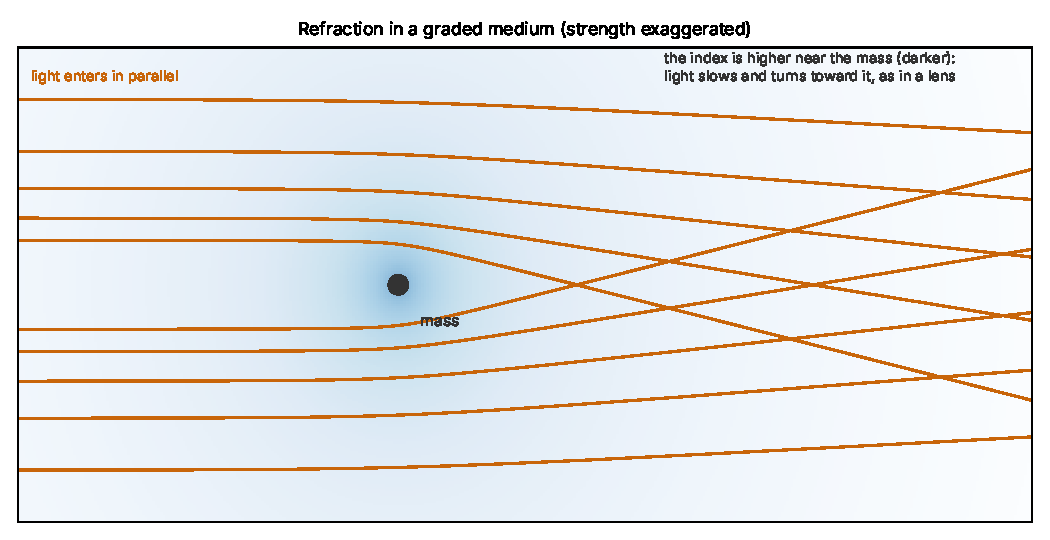
\includegraphics[width=0.92\linewidth]{fig10-1-refraction.pdf}
\caption{Light refracted by a graded medium. Parallel rays pass a mass whose surrounding index is raised (darker shading); each ray slows on its nearer side and turns toward the mass, and rays passing close are turned most. The strength is exaggerated so that the turning can be seen; past the Sun it is 1.75 arcseconds.}\label{fig:refraction}
\end{figure}

\argm{The standard account calculates lensing this way.} Eddington described the bending of starlight in 1920 as the effect of a medium of graded index around the Sun,\fn{eddington1920} and the standard textbook on gravitational lenses derives the bending and the delay from exactly such an index.\fn{schneider1992} Figure~\ref{fig:refraction} shows the mechanism. Light is not bent by a force acting on it across empty space. It is refracted by the medium it travels through.

\argm{Mirages and lenses work the same way.} Over hot ground, air near the surface is thinner and its index lower, and light from the sky is turned upward into the eye: a mirage. A glass lens bends light by slowing it more in its thick middle than at its thin edge. A mass surrounds itself with a graded index in the medium, highest nearest the mass, and light passing it is turned toward it. In each case the cause is the same: the speed of light changes across the wavefront, and the wavefront turns.

\subsection{What is measured}

\argm{The bending and the slowing are measured, and agree.} Radio waves passing the Sun are bent by the amount the index gives, confirmed by radio interferometry from 1979 to 1999 to about 4 parts in 10,000.\fn{shapiro2004} Radar sent past the Sun to the planets returns late by the amount the same index gives: light's effective speed there is $c/n$ (Part 28). Radio waves and visible light are bent alike (Part 27).\fn{rashadaPart27} The index belongs to the medium, not to the light.

\argm{Light passing a lensed galaxy takes paths of different length through different index,} and arrives at different times. The time difference between images of a lensed quasar has two parts: the difference in the paths' lengths, and the difference in how long each spends in the region of raised index (Part 9).\fn{rashadaPart9} Both belong to the same picture: a wave crossing a graded medium.

\subsection{The proposals, tested}

\argm{A moving lens bends light where it is.} In 2002 Fomalont and Kopeikin measured the bending of a quasar's radio waves as Jupiter passed in front of it. The bending depended on Jupiter's position and motion as the light passed, measured to about 20 per cent.\fn{fomalont2003} What the measurement shows about the speed of gravity is debated. In GPT \hypm{the medium's pattern moves with the body} that sets it up (Part 16),\fn{rashadaPart16} so a moving lens bends light according to where its pattern is.

\argm{A rotating lens bends light unevenly.} Near a spinning mass, light passing on the side moving toward it is bent differently from light on the side moving away. General relativity predicts this, and the effect is far too small to measure past the Sun or a planet; near spinning black holes it shapes the images of their surroundings. In GPT \hypm{the unevenness is the medium's swirl} (Part 16), the same swirl Gravity Probe B measured around the Earth.

\argm{Gravity does not rotate polarisation.} A lens turns the direction of light; to first order it leaves the direction of its polarisation unchanged.\fn{faraoni1993} Where the polarisation of two images of one radio source differs, the difference is traced to magnetised plasma in the lensing galaxy, which turns polarisation by an amount that depends on wavelength; gravity's bending does not depend on wavelength at all.\fn{patnaik1999} A twist of polarisation by the medium's gradient alone is not seen.

\openm{Interference between lensed images} is owed. Where two images of one source differ in path by less than the length over which the waves stay in step, they can interfere. This is expected for gravitational waves lensed by galaxies, whose waves stay in step over great lengths. It has not yet been seen, and finer structure in how lensed light layers is not expected beyond what the index gives.

\section{Clocks and Redshift}

\subsection{The clock law}

\begin{hypbar}
\textbf{A clock is slowed by the medium streaming past it.} Time is the rate of a structure's internal change (Part 18).\footnotemark{} A clock is a structure of the medium's waves, and every cycle of it is carried by exchanges with the medium. Where the medium streams past the clock, those exchanges take longer and every cycle slows: compared with a clock far away, its rate is $\sqrt{P/P_0} = \sqrt{1 - w^2/c^2}$, where $w$ is the speed of the medium past it (Part 14).\footnotemark{} Near a mass the inflow is faster, the count of gravitons is higher and their active pressure is lower: a clock deeper in the well is in a denser, faster stream of the medium, and runs slower.
\end{hypbar}
\addtocounter{footnote}{-1}\footnotetext{\citealp{rashadaPart18}.}\stepcounter{footnote}\footnotetext{\citealp{rashadaPart14}.}

\argm{Gravitational and motional slowing are one effect.} The medium streaming past a clock may be the inflow, the clock's own motion through the medium, or both; the clock responds to the total. GPS clocks show it: their gain from height and their loss from speed come out together as 38.5 microseconds a day (Part 9). In 1971 Hafele and Keating flew atomic clocks around the world: the clocks flown eastward, moving faster through the medium, lost 59 nanoseconds against the ground; those flown westward gained 273.\fn{hafele1972}

\argm{The redshift is the difference between clocks.} A source deep in a mass's well emits light at its own rhythm, slowed by the faster stream of the medium there. The light carries that rhythm upward unchanged, and arrives where clocks run faster: compared with them, it is red. Pound and Rebka measured it up a 22.5-metre tower in 1960.\fn{pound1960} The light is not drained of energy on its way up; the clocks at the two ends differ.\fn{okun2000} The ratio of frequencies is the ratio of clock rates: $\nu_{\text{received}}/\nu_{\text{emitted}} = \sqrt{P_{\text{source}}/P_{\text{receiver}}}$.

\subsection{Maps of the medium, from clocks}

\argm{Clocks now map the medium's inflow.} Because a clock's rate follows the inflow where it stands, a precise enough clock is a map of the Earth's gravity: clock rates and gravity maps are two readings of one quantity. Optical clocks detect the change in rate from a 450-metre tower,\fn{takamoto2020} from the mountains above a tunnel through the Alps,\fn{grotti2018} and across a single millimetre of atoms.\fn{bothwell2022} Geodesists now use clocks to measure heights, and gravity maps to predict clock rates: the use of gravimetric maps to estimate local time dilation is practice. Near large masses and dense rock, clocks change rate by exactly what the inflow gives.

\section{Tests Proposed, and Their Results}

\begin{figure}[t]\centering
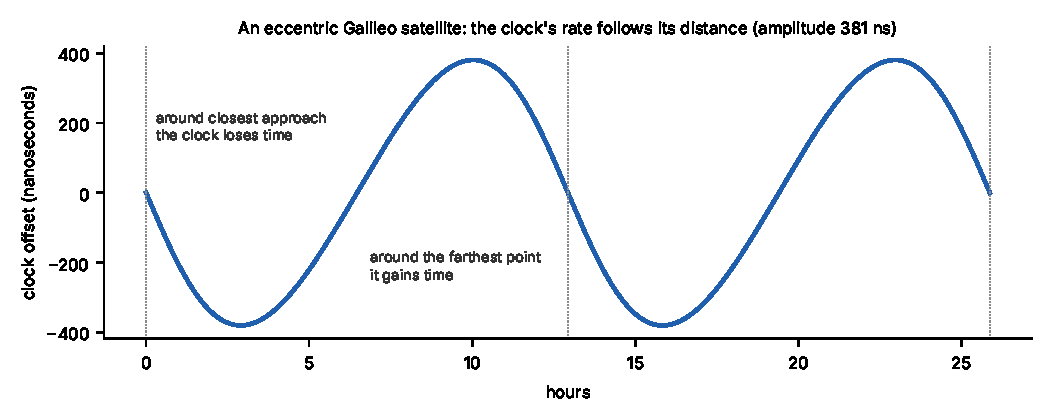
\includegraphics[width=0.92\linewidth]{fig10-2-galileo.pdf}
\caption{A clock in an elongated orbit. Two Galileo navigation satellites, placed by mistake in orbits that carry them between about 17,000 and 26,000 kilometres from the Earth's surface, lose time around closest approach, where the inflow is faster and they move faster through it, and gain it around the farthest point. Their clocks follow this curve, swinging by 380 nanoseconds each orbit; the measured swing matches it to a few parts in 100,000.}\label{fig:galileo}
\end{figure}

GPT proposes four tests of its clock law. Each has now been made, by others and for their own reasons. Table~\ref{tab:tests} summarises them.

\begin{table}[t]\centering\small
\caption{Tests of the clock law proposed in this paper, and their results.}
\begin{tabularx}{\linewidth}{@{}>{\raggedright}p{0.2\linewidth} >{\raggedright}p{0.3\linewidth} X@{}}\toprule
\textbf{Test} & \textbf{What GPT expects} & \textbf{Result}\\\midrule
Decay rates & every decaying particle slowed by the same factor as every clock & muons at 29 times their rest rate of decay slowed by exactly that factor \citep{bailey1977}; no yearly change with the Earth's distance from the Sun \citep{pomme2016}\\
Clocks in elongated orbits & slower near closest approach, by the inflow and speed there & Galileo satellites: as expected, to a few parts in 100,000 \citep{delva2018,herrmann2018}\\
Clocks in different settings & rate set by the medium streaming past, whatever the clock's construction & optical, atomic, nuclear and muon clocks all slow alike; rate across 1 mm resolved \citep{bothwell2022}\\
Timing of pulsars & signals from regions of strong flow, and waves of the medium, show in timing & binary pulsar timing as expected \citep{weisberg2016,kramer2021}; evidence for a background of waves of the medium \citep{agazie2023}\\\bottomrule
\end{tabularx}\label{tab:tests}\end{table}

\argm{Decaying particles are clocks.} Muons stored in a ring at 99.94 per cent of the speed of light decay 29.3 times more slowly than muons at rest, as the clock law gives, to about one part in a thousand.\fn{bailey1977} A muon's decay is a clock like any other, slowed by the medium streaming past it by the common factor. It was once reported that radioactive decay rates change through the year as the Earth's distance from the Sun changes.\fn{jenkins2009} Careful measurements of many kinds of decay, over years, found no such change: any yearly variation is smaller than a few parts in 100,000, and for the steadiest sources a few parts in a million.\fn{pomme2016} The medium changes decay rates only as it changes every clock.

\argm{Clocks in elongated orbits were tested by accident.} In 2014 two satellites of Europe's Galileo navigation system were launched into elongated orbits instead of circular ones. Their clocks swing ahead and behind as they move in and out, by 380 nanoseconds each orbit (Figure~\ref{fig:galileo}): slower around closest approach, where the inflow is faster and the satellite moves faster through it, as GPT expects. Two teams, analysing three years of data, found the swing matches the expected amount to a few parts in 100,000.\fn{delva2018}\textsuperscript{,}\fn{herrmann2018} No extra slowing at closest approach, beyond the clock law, was found.

\argm{Pulsars are timed to a ten-millionth of a second over decades.} In pairs, they show their companions' clock effects, the slowing of their signals past the companion, and the loss of energy to waves of the medium, all as expected.\fn{kramer2021} Timed together across the sky, they show a common wandering of their arrival times with the pattern expected from a background of slow waves of the medium passing the Earth: the NANOGrav collaboration found evidence for it at about three standard deviations in 2023, and other arrays agree.\fn{agazie2023} In GPT \hypm{this background is the medium itself ringing} with the waves of countless pairs of giant black holes.

\section{The Medium's Response to Sudden Change}

\subsection{The snapback effect}

When a mass changes suddenly, through a collapse, a collision or an explosion, the medium around it must change too. The medium cannot change everywhere at once.

\begin{hypbar}
\textbf{The medium re-settles, and the re-settling travels.} A sudden change in a mass changes its inflow, and the change spreads outward through the medium at the speed of its waves, $c$. Where the change is violent, the medium overshoots and rings before it settles: the snapback effect. It is the response of a real medium with inertia and stiffness, not an instantaneous adjustment of geometry.
\end{hypbar}

\subsection{What is measured}

\argm{Changes in gravity travel at the speed of light.} When two neutron stars merged in 2017, the change in the medium arrived together with the light, after 130 million years, to within a few parts in $10^{15}$.\fn{abbott2017speed}

\begin{figure}[t]\centering
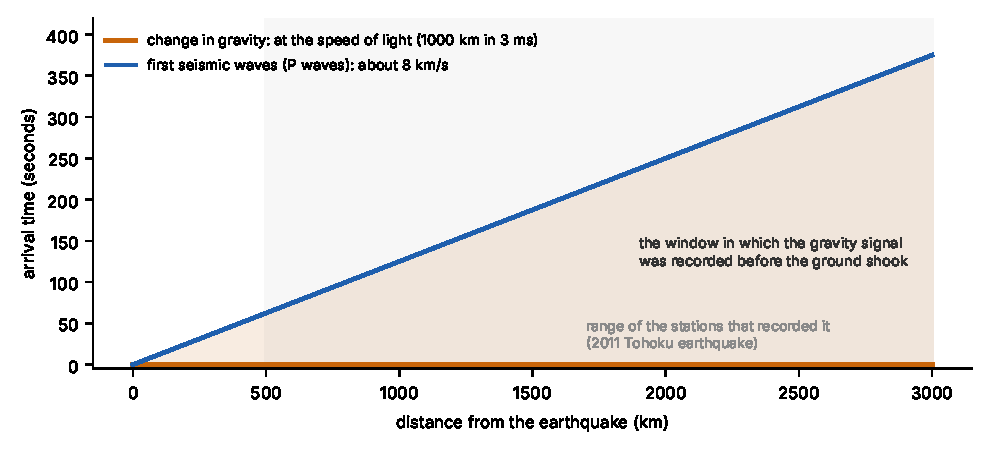
\includegraphics[width=0.9\linewidth]{fig10-3-pegs.pdf}
\caption{The medium responds first. When the 2011 Tohoku earthquake moved a vast mass of rock, the change in gravity spread at the speed of light, reaching a station 1,000 kilometres away in three thousandths of a second; the first seismic waves took two minutes. Seismometers and gravimeters 500 to 3,000 kilometres away recorded the gravity signal in the window between.}\label{fig:pegs}
\end{figure}

\argm{A great earthquake's change in gravity was recorded before the ground shook.} The magnitude 9.1 earthquake off Japan in 2011 moved an immense mass of rock in a few minutes. The change in gravity this caused spread at the speed of light. A gravimeter 500 kilometres away recorded it before any seismic wave arrived;\fn{montagner2016} about ten seismometers 500 to 3,000 kilometres away recorded it too, a station 1,000 kilometres away more than two minutes before the shaking (Figure~\ref{fig:pegs}).\fn{vallee2017} Satellites mapping the Earth's gravity measured the lasting change the earthquake left behind.\fn{matsuo2011} The medium responded to the mass's sudden change at once, at the speed of its waves, everywhere the instruments could see.

\argm{After a violent change, the medium rings and settles.} Two black holes merging leave the medium around the new black hole ringing at frequencies set by its mass and spin; LIGO recorded the ringing die away in milliseconds.\fn{isi2019} No repeated ``echoes'', which a reflecting surface would produce, have been found.\fn{abbott2021echo}

\openm{Whether the medium is left permanently shifted} after a wave passes, a ``memory'' that general relativity also predicts, is not yet measured.\fn{hubner2020}

\section{Galaxies}

Part 9 sets out the measurements: galaxies rotate as their visible matter says, above one acceleration scale, $a_0$, which GPT reads as the relaxation boundary of each mass in the medium. In GPT gravity is not an attraction from the centre but the medium's inflow, and the boundary is set by the visible mass that is there. Three further cases test the account.

\argm{Light around galaxies follows the same relation as orbits.} Weak lensing around galaxies shows the same flat speeds and the same relation between visible mass and speed as their rotation, out to hundreds of kiloparsecs.\fn{mistele2024} A galaxy's effect on light and on orbits is one effect, as it must be if both are the medium's.

\argm{Tidal dwarf galaxies are a challenge.} Small galaxies form from the gas torn out when large galaxies collide. Whatever the standard account's dark matter is, it should not be carried into these, and early measurements seemed to show more mass than their gas and stars.\fn{bournaud2007} Later, more careful measurements found their rotation consistent with their visible mass alone, and found them lying off the relation that other galaxies follow.\fn{lelli2015} If they are settled discs, that is a challenge for any account with a universal $a_0$, GPT's included. They have turned less than once since they formed, so whether they are settled is itself open.

\openm{The Bullet Cluster is owed.} Two clusters of galaxies have passed through each other. Their hot gas, most of their visible mass, collided and lagged behind; their galaxies passed through. The bending of background light follows the galaxies, not the gas.\fn{clowe2006} In GPT \hypm{a mass's pattern in the medium moves with it} (Part 16), so the pattern around the galaxies may have carried on with them while the gas was stopped. Whether this gives the measured lensing, in size and in place, is not yet worked out.

\section{What Remains to Be Derived}

\begin{itemize}
\item \openm{Interference between lensed images} of gravitational waves, and its size.
\item \openm{The medium's memory} after a wave passes.
\item \openm{The Bullet Cluster's lensing} from patterns that move with their galaxies.
\item \openm{Tidal dwarf galaxies,} once their state is settled.
\end{itemize}

\section*{Conclusion}
\addcontentsline{toc}{section}{Conclusion}

Each of the four ideas has become a measurement. Light is refracted by the medium's graded index: bent, slowed and delayed by one cause, as the standard account's own calculations show, with its polarisation untouched by gravity. Clocks are slowed by the medium streaming past them, whatever the reason for the streaming; the redshift is the difference between clocks; and clocks now map the inflow they sit in. The tests GPT proposed have been made: decaying muons slowed by exactly the clock factor, no yearly change in decay with the Sun's distance, Galileo clocks swinging in their elongated orbits as expected, and pulsars timed across decades showing the medium's waves. When a mass changes suddenly, the medium responds at the speed of light, as the great earthquake of 2011 showed before the ground shook, and after a violent change it rings and settles. Galaxies and their lensing follow one relation; tidal dwarfs and the Bullet Cluster are the cases still owed. With the Graviton Pressure Theory, we do not need to see the invisible. We need only to understand the medium that was there all along.

\clearpage
\section*{Changes in the Second Edition}
\addcontentsline{toc}{section}{Changes in the Second Edition}

This list records what changed from the first edition and why. Changes to the argument alter what the paper claims or how it supports a claim; clarifications improve wording, sources or presentation and leave the argument as it was.

\subsection*{Changes to the argument}
\begin{itemize}
\item \textbf{Lensing.} The index $n_g = 1 + \beta P_g$, with pressure rising toward a mass, is replaced by $n = P_0/P \approx 1 + 2GM/c^2r$: the active pressure is lower near a mass and the index higher (Part 23). Lensing as refraction, the mirage and glass analogies, and light's effective speed $c/n$ are kept. ``Not because of a longer path'' is restated: the delay between lensed images has both parts, path length and time in the raised index.
\item \textbf{Lensing predictions.} Asymmetric bending near rotating or moving bodies is kept and restated as the medium's swirl and moving pattern, with the Jupiter measurement. Polarisation rotation across gravitational gradients is withdrawn: gravity does not rotate polarisation to first order, and observed differences between images are traced to plasma in the lens. ``Layered interference patterns'' revealing ``quantised tension stratification'' are withdrawn; interference between lensed images is kept as open.
\item \textbf{Redshift.} ``Phase coherence transformation'', in which the field drains the light's energy on the way up, and the formula $\Delta f \approx -f_0\,\Delta P_g/P_c$, are replaced: the redshift is the difference between the clocks at the two ends, $\nu_{\text{received}}/\nu_{\text{emitted}} = \sqrt{P_{\text{source}}/P_{\text{receiver}}}$.
\item \textbf{Time dilation.} The law $\Delta\tau/\Delta t = \sqrt{P_0/P}$ is inverted in the first edition and is corrected to $\sqrt{P/P_0}$. ``Temporal drag'' in a denser graviton field is kept: the count of gravitons is higher near a mass while their active pressure is lower, and the clock is slowed by the faster stream. The claim that GPT diverges from general relativity in strong fields is withdrawn: the inflow reproduces the same numbers at every strength (Part 23). ``GR breaks near singularities; GPT extends from quantum to cosmic'' is withdrawn as an unsupported comparison. The use of gravimetric maps to predict clock rates is kept, and is now practice.
\item \textbf{Tests.} Each proposed test is reported with its result: decay rates (muons; the yearly-variation claim and its refutation), elliptical orbits (Galileo), photon clocks (optical clocks across a millimetre; ``pressure-tunable media'' and ``graviton analog field injectors'' are withdrawn), and pulsar timing. Expectations of deviations beyond the clock law are withdrawn: none were found.
\item \textbf{Snapback.} Kept as the medium re-settling at $c$ and ringing, and supported by the earthquake gravity signal, the 2017 merger and the measured ringdown. The ``observed anomalies'' (spacecraft trajectory changes near transient disturbances, lunar orbit changes after solar mass ejections, lensing changes after supernovae) are withdrawn: no source was given, and none is known. The claim that general relativity has no response to sudden change is withdrawn: it predicts waves at $c$, ringdown and memory.
\item \textbf{Galaxies.} The rotation-curve account defers to Part 9's relaxation boundary. ``Pressure basins'' formed by mass ``blocking'' the flow are withdrawn: shielding is bounded far below what this needs (Part 15). The dwarf and tidal-dwarf claim is reversed: tidal dwarfs show no excess mass and lie off the relation, a challenge. ``Lack of lensing consistency'' is replaced by lensing following the same relation as rotation. The Bullet Cluster's ``pressure lag'' is kept as the medium's pattern moving with its galaxies, marked as owed.
\end{itemize}

\subsection*{Clarifications}
\begin{itemize}
\item ``Light is coherence, not a photon particle'' is restated in line with Part 28, where single-photon behaviour is kept as an open question.
\item Collaborators named as ideal partners are removed.
\item Three figures and a table of tests are added; sources are added for every measurement.
\item The cross-references are renumbered.
\end{itemize}

\bibliography{part10}
\end{document}
